%  The "autowc" option automatically inserts a word count 
%  on the title page, using texcount. (The "Frontmatter" 
%  on the title page and reference list are omitted.)
%  NOTE THAT THIS WILL ONLY WORK IF YOU HAVE  
%  INSTALLED TEXCOUNT, AND HAVE ENABLED --shell-escape
%  OR --enable-write18. (These will work on Overleaf.)
%  If you get an error about "texcount not found", delete
%  the autowc option, and manually specify the wordcount 
%  with \totalwordcount{xxx}.
% autowc may cause longer compilation time. You can 
% disable it first while actively editing, and only
% enable it when you're ready to take stock and check
% on your work.
\documentclass[autowc]{CUP-JNL-PPS}

% Use these lines if you want to provide a manual word count or if you're not using texcount.
% \documentclass{CUP-JNL-PPS}
% \totalwordcount{500}

%%%% Packages
\usepackage{latexsym}
\usepackage{graphicx}
\usepackage{multicol,multirow}
\usepackage{amsmath,amssymb,amsfonts}
\usepackage{mathrsfs}
\usepackage{amsthm}
\usepackage{rotating}
\usepackage{appendix}
\usepackage[authoryear]{natbib}
\usepackage{ifpdf}
\usepackage[T1]{fontenc}
\usepackage[type1,lining]{ebgaramond}
\usepackage[type1,lining]{sourcesanspro}
\usepackage{newtxmath}
\usepackage{textcomp}%
\usepackage{xcolor}%
\usepackage{hyperref}
\usepackage{lipsum}
%%%%

%\articletype{RESEARCH ARTICLE}
\jname{Perspectives on Politics}
%\artid{20}
\jyear{2021}
\jvol{4}
%\jissue{1}
\jdoi{10.1017/pps.2021.xx}
%\raggedbottom

%\usepackage{showframe}

\begin{document}

%% When using autowc (automatic wordcount, you can use %TC:ignore and %TC:endignore blocks to mark regions of text that should be omitted from counting.)
%TC:ignore
\begin{Frontmatter}
\title[Article Title]{Sample for Article Title\thanks{Author N. \authororcid{0000-0002-8514-4315} Professor of Political Science at Princeton University. Her
research targets the intersection of politics and belonging in
relation to immigrant integration issues and national identity, from the point of view of minorities and majorities alike.

They thank the following research assistants for their work on this article: Author Name2, Author Name3. They also thank the incredibly generous and thoughtful reviewers, who engaged in the best possible way with the arguments they have offered here. The article is much stronger for their work. }}

\author{Author Name1, University, Country}
\author{Author Name2, University, Country}
\author{Author Name3, University, Country}

\abstract{Abstracts should be 250 words. It must be able to stand alone and so cannot contain citations to the paper's references, equations, etc. An abstract must consist of a single paragraph and be concise. Because of online formatting, abstracts must appear as plain as possible.}

\end{Frontmatter}
%TC:endignore


\dropcap{M}axime mollitia, molestiae quas vel sint commodi repudiandae consequuntur voluptatum laborum
numquam blanditiis harum quisquam eius sed odit fugiat iusto fuga praesentium
optio, eaque rerum! Provident similique accusantium nemo autem. Veritatis
obcaecati tenetur iure eius earum ut molestias architecto voluptate aliquam
nihil, eveniet aliquid culpa officia aut! Impedit sit sunt quaerat, odit,
tenetur error, harum nesciunt ipsum debitis quas aliquid. Reprehenderit,
quia. Quo neque error repudiandae fuga? Ipsa laudantium molestias eos
sapiente officiis modi at sunt excepturi expedita sint? Sed quibusdam
recusandae alias error harum maxime adipisci amet laborum. Perspiciatis
minima nesciunt dolorem! Officiis iure rerum voluptates a cumque velit
quibusdam sed amet tempora. Sit laborum ab, eius fugit doloribus tenetur
fugiat, temporibus enim commodi iusto libero magni deleniti quod quam
consequuntur! Commodi minima excepturi repudiandae velit hic maxime
doloremque. Quaerat provident commodi consectetur veniam similique ad
earum omnis ipsum saepe, voluptas, hic voluptates pariatur est explicabo
fugiat, dolorum eligendi quam cupiditate excepturi mollitia maiores labore
suscipit quas? Nulla, placeat. Voluptatem quaerat non architecto ab laudantium
modi minima sunt esse temporibus sint culpa, recusandae aliquam numquam
totam ratione voluptas quod exercitationem fuga. Possimus quis earum veniam
quasi aliquam eligendi, placeat qui corporis!

Lorem ipsum dolor sit amet consectetur adipisicing elit. Maxime mollitia,
molestiae quas vel sint commodi repudiandae consequuntur voluptatum laborum
numquam blanditiis harum quisquam eius sed odit fugiat iusto fuga praesentium
optio, eaque rerum! Provident similique accusantium nemo autem. Veritatis
obcaecati tenetur iure eius earum ut molestias architecto voluptate aliquam
nihil, eveniet aliquid culpa officia aut! Impedit sit sunt quaerat, odit,
tenetur error, harum nesciunt ipsum debitis quas aliquid. Reprehenderit,
quia. Quo neque error repudiandae fuga? Ipsa laudantium molestias eos
sapiente officiis modi at sunt excepturi expedita sint? Sed quibusdam
recusandae alias error harum maxime adipisci amet laborum. Perspiciatis
minima nesciunt dolorem! Officiis iure rerum voluptates a cumque velit
quibusdam sed amet tempora. Sit laborum ab, eius fugit doloribus tenetur
fugiat, temporibus enim commodi iusto libero magni deleniti quod quam
consequuntur! Commodi minima excepturi repudiandae velit hic maxime
doloremque. Quaerat provident commodi consectetur veniam similique ad
earum omnis ipsum saepe, voluptas, hic voluptates pariatur est explicabo
fugiat, dolorum eligendi quam cupiditate excepturi mollitia maiores labore
suscipit quas? Nulla, placeat. Voluptatem quaerat non architecto ab laudantium
modi minima sunt esse temporibus sint culpa, recusandae aliquam numquam
totam ratione voluptas quod exercitationem fuga. Possimus quis earum veniam
quasi aliquam eligendi, placeat qui corporis!

Lorem ipsum dolor sit amet consectetur adipisicing elit. Maxime mollitia,
molestiae quas vel sint commodi repudiandae consequuntur voluptatum laborum
numquam blanditiis harum quisquam eius sed odit fugiat iusto fuga praesentium
optio, eaque rerum! Provident similique accusantium nemo autem. Veritatis
obcaecati tenetur iure eius earum ut molestias architecto voluptate aliquam
nihil, eveniet aliquid culpa officia aut! Impedit sit sunt quaerat, odit,
tenetur error, harum nesciunt ipsum debitis quas aliquid. Reprehenderit,
quia. Quo neque error repudiandae fuga? Ipsa laudantium molestias eos
sapiente officiis modi at sunt excepturi expedita sint? Sed quibusdam
recusandae alias error harum maxime adipisci amet laborum. Perspiciatis
minima nesciunt dolorem! Officiis iure rerum voluptates a cumque velit
quibusdam sed amet tempora. Sit laborum ab, eius fugit doloribus tenetur
fugiat, temporibus enim commodi iusto libero magni deleniti quod quam
consequuntur! Commodi minima excepturi repudiandae velit hic maxime
doloremque. Quaerat provident commodi consectetur veniam similique ad
earum omnis ipsum saepe, voluptas, hic voluptates pariatur est explicabo
fugiat, dolorum eligendi quam cupiditate excepturi mollitia maiores labore
suscipit quas? Nulla, placeat. Voluptatem quaerat non architecto ab laudantium
modi minima sunt esse temporibus sint culpa, recusandae aliquam numquam
totam ratione voluptas quod exercitationem fuga. Possimus quis earum veniam
quasi aliquam eligendi, placeat qui corporis!

Lorem ipsum dolor sit amet consectetur adipisicing elit. Maxime mollitia,
molestiae quas vel sint commodi repudiandae consequuntur voluptatum laborum
numquam blanditiis harum quisquam eius sed odit fugiat iusto fuga praesentium
optio, eaque rerum! Provident similique accusantium nemo autem. Veritatis
obcaecati tenetur iure eius earum ut molestias architecto voluptate aliquam
nihil, eveniet aliquid culpa officia aut! Impedit sit sunt quaerat, odit,
tenetur error, harum nesciunt ipsum debitis quas aliquid. Reprehenderit,
quia. Quo neque error repudiandae fuga? Ipsa laudantium molestias eos
sapiente officiis modi at sunt excepturi expedita sint? Sed quibusdam
recusandae alias error harum maxime adipisci amet laborum. Perspiciatis
minima nesciunt dolorem! Officiis iure rerum voluptates a cumque velit
quibusdam sed amet tempora. Sit laborum ab, eius fugit doloribus tenetur
fugiat, temporibus enim commodi iusto libero magni deleniti quod quam
consequuntur! Commodi minima excepturi repudiandae velit hic maxime
doloremque. Quaerat provident commodi consectetur veniam similique ad
earum omnis ipsum saepe, voluptas, hic voluptates pariatur est explicabo
fugiat, dolorum eligendi quam cupiditate excepturi mollitia maiores labore
suscipit quas? Nulla, placeat. Voluptatem quaerat non architecto ab laudantium
modi minima sunt esse temporibus sint culpa, recusandae aliquam numquam
totam ratione voluptas quod exercitationem fuga. Possimus quis earum veniam
quasi aliquam eligendi, placeat qui corporis!

Lorem ipsum dolor sit amet consectetur adipisicing elit. Maxime mollitia,
molestiae quas vel sint commodi repudiandae consequuntur voluptatum laborum
numquam blanditiis harum quisquam eius sed odit fugiat iusto fuga praesentium
optio, eaque rerum! Provident similique accusantium nemo autem. Veritatis
obcaecati tenetur iure eius earum ut molestias architecto voluptate aliquam
nihil, eveniet aliquid culpa officia aut! Impedit sit sunt quaerat, odit,
tenetur error, harum nesciunt ipsum debitis quas aliquid. Reprehenderit,
quia. Quo neque error repudiandae fuga? Ipsa laudantium molestias eos
sapiente officiis modi at sunt excepturi expedita sint? Sed quibusdam
recusandae alias error harum maxime adipisci amet laborum. Perspiciatis
minima nesciunt dolorem! Officiis iure rerum voluptates a cumque velit
quibusdam sed amet tempora. Sit laborum ab, eius fugit doloribus tenetur
fugiat, temporibus enim commodi iusto libero magni deleniti quod quam
consequuntur! Commodi minima excepturi repudiandae velit hic maxime
doloremque. Quaerat provident commodi consectetur veniam similique ad
earum omnis ipsum saepe, voluptas, hic voluptates pariatur est explicabo
fugiat, dolorum eligendi quam cupiditate excepturi mollitia maiores labore
suscipit quas? Nulla, placeat. Voluptatem quaerat non architecto ab laudantium
modi minima sunt esse temporibus sint culpa, recusandae aliquam numquam
totam ratione voluptas quod exercitationem fuga. Possimus quis earum veniam
quasi aliquam eligendi.

\section[This is an A Head]{This is an A head this is an A head this is an A head}
\lipsum[1]

\subsection{This is a B head this is a B head this is a B head this is a B head}

\lipsum[2]

\subsubsection{This is a C head this is a C head}

\lipsum[3]

\section[This is an A Head]{This is an A head this is an A head this is an A head this is an~A~head}
\subsection{This is a B head this is a B head this is a B head this is a B head this is a B~head}
\subsubsection{This is a C head this is a C head this is a C head this is a C head}
\lipsum[4]
\begin{quote}
\textit{Heading.} Quaerat provident commodi consectetur veniam similique ad
earum omnis ipsum saepe, voluptas, hic voluptates pariatur est explicabo
fugiat, dolorum eligendi quam cupiditate excepturi mollitia maiores labore
suscipit quas? Nulla, placeat. Voluptatem quaerat non architecto ab laudantium
modi minima sunt esse temporibus sint culpa, recusandae aliquam numquam
totam ratione voluptas quod exercitationem fuga. Possimus quis earum veniam
quasi aliquam eligendi.\footnote{This is sample for footnote this is sample for footnote this is sample for footnote  this is sample for footnote this is sample for footnote.}%
\end{quote}%

Voluptatem quaerat non architecto ab laudantium
modi minima sunt esse temporibus sint culpa, recusandae aliquam numquam
totam ratione voluptas quod exercitationem fuga. Possimus quis earum veniam
quasi aliquam eligendi.
Voluptatem quaerat non architecto ab laudantium
modi minima sunt esse temporibus sint culpa, recusandae aliquam numquam
totam ratione. Possimus quis earum veniam
quasi aliquam eligendi.

Voluptatem quaerat non architecto ab laudantium
modi minima sunt esse temporibus sint culpa, recusandae aliquam numquam
totam ratione voluptas quod exercitationem fuga. Possimus quis earum veniam
quasi aliquam eligendi.
Voluptatem quaerat non architecto ab laudantium
modi minima sunt esse temporibus sint culpa, recusandae aliquam numquam
totam ratione voluptas quod exercitationem fuga. Possimus quis earum veniam
quasi aliquam eligendi.

Voluptatem quaerat non architecto ab laudantium
modi minima sunt esse temporibus sint culpa, recusandae aliquam numquam
totam ratione voluptas quod exercitationem fuga. Possimus quis earum veniam
quasi aliquam eligendi.
Voluptatem quaerat non architecto ab laudantium
modi minima sunt esse temporibus sint culpa, recusandae aliquam numquam
totam ratione voluptas quod exercitationem fuga. Possimus quis earum veniam
quasi aliquam eligendi.
Voluptatem quaerat non architecto ab laudantium
modi minima sunt esse temporibus sint culpa, recusandae aliquam numquam
totam ratione voluptas quod exercitationem fuga.


\section{Lists}

List in \LaTeX{} can be of three types: enumerate, itemize and description.
In each environments, new entry is added via the \verb+\item+ command.
Enumerate creates numbered lists, itemize creates bulleted lists and
description creates description lists.
\begin{enumerate}[1.]
\item First item in the number list.
\item Second item in the number list.
\item Third item in the number list.
\end{enumerate}
List in \LaTeX{} can be of three types: enumerate, itemize and description.
In each environments, new entry is added via the \verb+\item+ command.
\begin{itemize}
\item First item in the bullet list.
\item Second item in the bullet list.
\item Third item in the bullet list.
\end{itemize}


\section{Equations}

Equations in \LaTeX{} can either be inline or on-a-line by itself. For
inline equations use the \verb+$...$+ commands. Eg: The equation
$H\psi = E \psi$ is written via the command $H \psi = E \psi$.

For on-a-line by itself equations (with auto generated equation numbers)
one can use the equation or eqnarray environments \textit{D}.
\begin{equation}
\mathcal{L} = i {\psi} \gamma^\mu D_\mu \psi
    - \frac{1}{4} F_{\mu\nu}^a F^{a\mu\nu} - m {\psi} \psi
\label{eq1}
\end{equation}
where,
\begin{align}
D_\mu &=  \partial_\mu - ig \frac{\lambda^a}{2} A^a_\mu
\nonumber \\
F^a_{\mu\nu} &= \partial_\mu A^a_\nu - \partial_\nu A^a_\mu
    + g f^{abc} A^b_\mu A^a_\nu
\label{eq2}
\end{align}
Notice the use of \verb+\nonumber+ in the align environment at the end
of each line, except the last, so as not to produce equation numbers on
lines where no equation numbers are required. The \verb+\label{}+ command
should only be used at the last line of an align environment where
\verb+\nonumber+ is not used.
\begin{equation}
Y_\infty = \left( \frac{m}{\textrm{GeV}} \right)^{-3}
    \left[ 1 + \frac{3 \ln(m/\textrm{GeV})}{15}
    + \frac{\ln(c_2/5)}{15} \right]
\end{equation}
The class file also supports the use of \verb+\mathbb{}+, \verb+\mathscr{}+ and
\verb+\mathcal{}+ commands. As such \verb+\mathbb{R}+, \verb+\mathscr{R}+
and \verb+\mathcal{R}+ produces $\mathbb{R}$, $\mathscr{R}$ and $\mathcal{R}$
respectively.\footnote{This is sample for footnote this is sample for footnote this is sample for footnote  this is sample for footnote this is sample for footnote.}

Voluptatem quaerat non architecto ab laudantium
modi minima sunt esse temporibus sint culpa, recusandae aliquam numquam
totam ratione voluptas quod exercitationem fuga. Possimus quis earum veniam
quasi aliquam eligendi.
Voluptatem quaerat non architecto ab laudantium
modi minima sunt esse temporibus sint culpa, recusandae aliquam numquam
totam ratione voluptas quod exercitationem fuga. Possimus quis earum veniam
quasi aliquam eligendi.
Voluptatem quaerat non architecto ab laudantium
modi minima sunt esse temporibus sint culpa, recusandae aliquam numquam
totam ratione.
%% voluptas quod exercitationem fuga.

\section{Figures}

As per the \LaTeX\ standards eps images in \verb!latex! and pdf/jpg/png images in
\verb!pdflatex! should be used. This is one of the major differences between \verb!latex!
and \verb!pdflatex!. The images should be single page documents. The command for inserting images
for latex and pdflatex can be generalized. The package that should be used
is the graphicx package.

\begin{figure}[t]%
\FIG{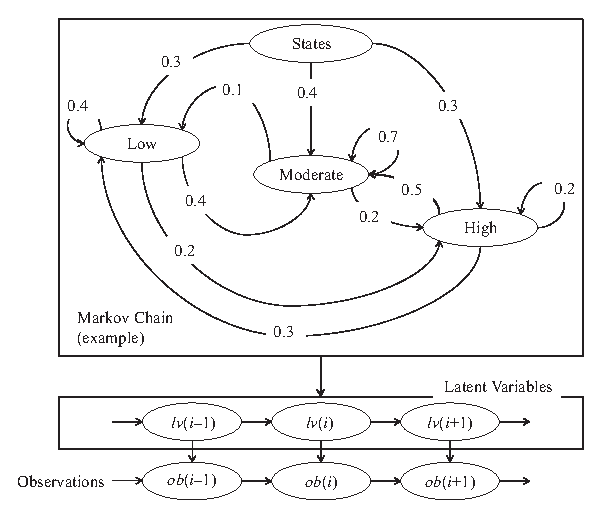
\includegraphics[width=.75\columnwidth]{Fig}}
{\caption{This is an example of caption this is an example of caption  this is an example of caption this is an example of caption}
\label{fig1}}
\end{figure}



\section{Tables}

Tables can be inserted via the normal table and tabular environment. To put
footnotes inside tables one has to use the additional ``fntable" environment
enclosing the tabular environment. The footnote appears just below the table
itself.

\begin{table}[t]
\tabcolsep=0pt%
\TBL{\caption{Tables which are too long to fit,
should be written using the ``table*'' environment\label{tab2}}}
{\begin{fntable}
\begin{tabular*}{\textwidth}{@{\extracolsep{\fill}}lcccccc@{}}\toprule%
 & \multicolumn{3}{@{}c@{}}{\TCH{Element 1}}& \multicolumn{3}{@{}c@{}}{\TCH{Element 2\smash{\footnotemark[1]}}}
 \\\cmidrule{2-4}\cmidrule{5-7}%
\TCH{Project} & \TCH{Energy} & \TCH{$\boldsymbol{\sigma_{\text{calc}}}$} & \TCH{$\boldsymbol{\sigma_{\text{expt}}}$} &
\TCH{Energy} & \TCH{$\boldsymbol{\sigma_{\text{calc}}}$} & \TCH{$\boldsymbol{\sigma_{\text{expt}}}$} \\\midrule
\TCH{Stage 3}&990 A &168 &47$\pm$12 &78 A &66 &39$\pm$10\\
{\TCH{Stage 4}}&500 A &961 &22$\pm$10 &90 A &68 &92$\pm$40\\
\botrule
\end{tabular*}%
\footnotetext[]{{Note:} This is an example of table footnote this is an example of table footnote this is an example of table footnote this is an example of~table footnote this is an example of table footnote}
\footnotetext[1]{This is an example of table footnote}%
\end{fntable}}
\vspace*{7pt}
\end{table}



\section{Cross referencing}

Environments such as figure, table, equation, align can have a label
declared via the \verb+\label{#label}+ command. For figures and table
environments one should use the \verb+\label{}+ command inside or just
below the \verb+\caption{}+ command.  One can then use the
\verb+\ref{#label}+ command to cross-reference them. As an example, consider
the label declared for Figure \ref{fig1} which is
\verb+\label{fig1}+. To cross-reference it, use the command
\verb+ Figure \ref{fig1}+, for which it comes up as
``Figure \ref{fig1}''.
The reference citations should used as per the ``natbib'' packages. Some sample citations:  \cite{bib1} and \citep{bib1,bib2,bib3,bib4,bib5}.

\begin{appendix}\appheader
\section{Appendix. Title for Appendix Section}\label{appendixA}
Appendix text here.
\end{appendix}

\theendnotes

\section{Conclusion}

Some Conclusions here.



\begin{Backmatter}

%%%\paragraph{Acknowledgments}
%%%We are grateful for the technical assistance of A. Author.
%%%
%%%
%%%\paragraph{Funding Statement}
%%%This research was supported by grants from the <funder-name><doi>(<award ID>); <funder-name><doi>(<award ID>).
%%%
%%%\paragraph{Competing Interests}
%%%A statement about any financial, professional, contractual or personal relationships or situations that could be perceived to impact the presentation of the work --- or `None' if none exist
%%%
%%%\paragraph{Data Availability Statement}
%%%A statement about how to access data, code and other materials allowing users to understand, verify and replicate findings --- e.g. Replication data and code can be found in Harvard Dataverse: \verb+\url{https://doi.org/link}+.
%%%
%%%\paragraph{Ethical Standards}
%%%The research meets all ethical guidelines, including adherence to the legal requirements of the study country.
%%%
%%%\paragraph{Author Contributions}
%%%Please provide an author contributions statement using the CRediT taxonomy roles as a guide {\verb+\url{https://www.casrai.org/credit.html}+}. Conceptualization: A.A; A.B. Methodology: A.A; A.B. Data curation: A.C. Data visualisation: A.C. Writing original draft: A.A; A.B. All authors approved the final submitted draft.
%%%
%%%\paragraph{Supplementary Material}
%%%State whether any supplementary material intended for publication has been provided with the submission.

\begin{thebibliography}{}
\bibitem[Ananin and Mironov (2000)]{bib1}
{Ananin, Beth, and Mironov, Antony}. 2000. ``The moduli space of $2$-dimensional algebras'', \textit{Comm. Algebra} {28}(9),  {4481}--{4488}.

\bibitem[Bai and Meng (2001)]{bib2}
{Bai, Clifton, and Meng, Dyck}. 2001. ``The classification of Novikov algebras in low dimension'',  \textit{J. Phys. A: Math. Gen.} {34}, {1581}--{1594}.

\bibitem[Ca\~{n}ete and Khudoyberdiyev (2013)]{bib3}
{Ca\~{n}ete, Enderson, and Khudoyberdiyev, Angus}. 2013. ``The classification of $4$-dimensional Leibniz algebras'',  \textit{Linear Algebra and its Applications}  {439}(1), {273}--{288}.

\bibitem[Goze and Remm (2011)]{bib4}
{Goze, Michael, and Remm, Edward}. 2011.  ``$2$-dimensional algebras'',  \textit{Afr. J. Math. Phys.} {10}(1),  {81}--{91}.

\bibitem[Petersson (2000)]{bib5}
{Petersson, Hentry}. 2000. ``The classification of two-dimensional nonassociative algebras'',  \textit{Results Math} {37}, no. 1-2,  {120}--{154}.

\end{thebibliography}

\end{Backmatter}


\end{document}
